\documentclass{standalone}
\usepackage{tikz}
\usepackage{pgfplots}
\usetikzlibrary{positioning,3d,decorations.markings,calc}
\pgfplotsset{compat=1.18}

\begin{document}
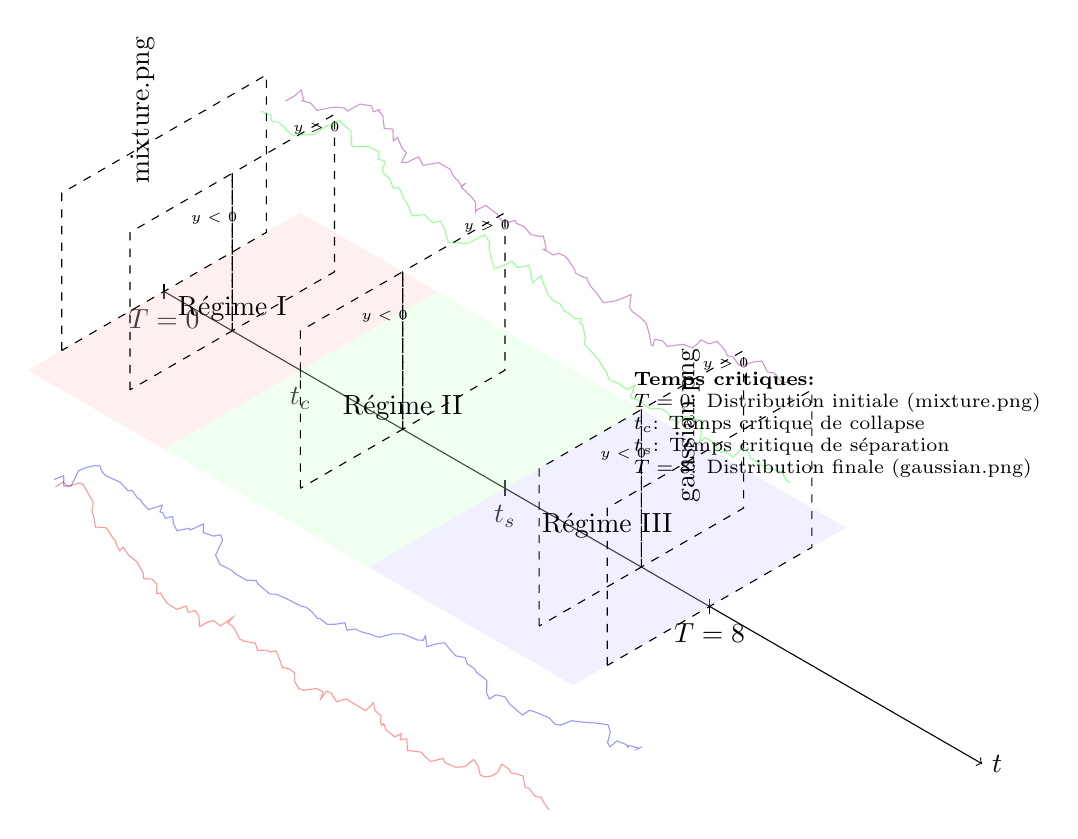
\begin{tikzpicture}[
    x={(0.866cm,-0.5cm)},
    y={(0.866cm,0.5cm)},
    z={(0cm,1cm)}
]
    % Axe temporel
    \draw[->] (0,0,0) -- (12,0,0) node[right] {$t$};
    
    % Points temporels importants
    \draw (8,0,0.1) -- (8,0,-0.1) node[below] {$T=8$};
    \draw (5,0,0.1) -- (5,0,-0.1) node[below] {$t_s$};
    \draw (2,0,0.1) -- (2,0,-0.1) node[below] {$t_c$};
    \draw (0,0,0.1) -- (0,0,-0.1) node[below] {$T=0$};
    
    % Zones de régimes colorées
    \fill[blue!20,opacity=0.3] (8,-2,0) -- (8,2,0) -- (5,2,0) -- (5,-2,0) -- cycle; % Régime III
    \fill[green!20,opacity=0.3] (5,-2,0) -- (5,2,0) -- (2,2,0) -- (2,-2,0) -- cycle; % Régime II
    \fill[red!20,opacity=0.3] (2,-2,0) -- (2,2,0) -- (0,2,0) -- (0,-2,0) -- cycle; % Régime I
    
    % Labels des régimes
    \node[above] at (6.5,0,0) {Régime III};
    \node[above] at (3.5,0,0) {Régime II};
    \node[above] at (1,0,0) {Régime I};

    % Encarts pour les coupes aux extrémités (T=0 et T=8)
    % T=0
    \draw[dashed] (0,-1.5,0) -- (0,-1.5,2) -- (0,1.5,2) -- (0,1.5,0) -- cycle;
    \node[rotate=90, anchor=south] at (0,0,2.3) {mixture.png};
    
    % T=8
    \draw[dashed] (8,-1.5,0) -- (8,-1.5,2) -- (8,1.5,2) -- (8,1.5,0) -- cycle;
    \node[rotate=90, anchor=south] at (8,0,2.3) {gaussian.png};

    % Encarts pour les coupes (y,z) - maintenant divisés en y+ et y-
    % Régime I - y positif
    \draw[dashed] (1,0,0) -- (1,0,2) -- (1,1.5,2) -- (1,1.5,0) -- cycle;
    \node[anchor=south west, font=\tiny] at (1,0.75,2) {$y>0$};
    
    % Régime I - y négatif
    \draw[dashed] (1,-1.5,0) -- (1,-1.5,2) -- (1,0,2) -- (1,0,0) -- cycle;
    \node[anchor=north west, font=\tiny] at (1,-0.75,2) {$y<0$};
    
    % Régime II - y positif
    \draw[dashed] (3.5,0,0) -- (3.5,0,2) -- (3.5,1.5,2) -- (3.5,1.5,0) -- cycle;
    \node[anchor=south west, font=\tiny] at (3.5,0.75,2) {$y>0$};
    
    % Régime II - y négatif
    \draw[dashed] (3.5,-1.5,0) -- (3.5,-1.5,2) -- (3.5,0,2) -- (3.5,0,0) -- cycle;
    \node[anchor=north west, font=\tiny] at (3.5,-0.75,2) {$y<0$};
    
    % Régime III - y positif
    \draw[dashed] (7,0,0) -- (7,0,2) -- (7,1.5,2) -- (7,1.5,0) -- cycle;
    \node[anchor=south west, font=\tiny] at (7,0.75,2) {$y>0$};
    
    % Régime III - y négatif
    \draw[dashed] (7,-1.5,0) -- (7,-1.5,2) -- (7,0,2) -- (7,0,0) -- cycle;
    \node[anchor=north west, font=\tiny] at (7,-0.75,2) {$y<0$};

    % Trajectoire 1 (rouge)
    \draw[red,opacity=0.4] plot coordinates {
        (0,-1.593,-1.687) (0.08,-1.556,-1.601) (0.16,-1.569,-1.614) (0.24,-1.480,-1.571)
        (0.32,-1.506,-1.540) (0.40,-1.533,-1.567) (0.48,-1.519,-1.675) (0.56,-1.617,-1.707)
        (0.64,-1.674,-1.689) (0.72,-1.725,-1.769) (0.80,-1.642,-1.782) (0.88,-1.638,-1.862)
        (0.96,-1.669,-1.856) (1.04,-1.734,-1.835) (1.12,-1.768,-1.851) (1.20,-1.802,-1.746)
        (1.28,-1.803,-1.806) (1.36,-1.757,-1.875) (1.44,-1.745,-1.986) (1.52,-1.820,-1.975)
        (1.60,-1.778,-1.965) (1.68,-1.785,-1.982) (1.76,-1.868,-2.023) (1.84,-1.894,-1.963)
        (1.92,-1.875,-2.063) (2.00,-1.857,-2.085) (2.08,-1.895,-2.050) (2.16,-1.837,-1.997)
        (2.24,-1.884,-2.015) (2.32,-1.865,-1.960) (2.40,-1.892,-1.970) (2.48,-1.955,-2.038)
        (2.56,-1.909,-1.961) (2.64,-1.913,-1.904) (2.72,-1.893,-1.941) (2.80,-1.872,-1.854)
        (2.88,-1.874,-1.765) (2.96,-2.022,-1.719) (3.04,-2.018,-1.736) (3.12,-2.012,-1.848)
        (3.20,-2.025,-1.828) (3.28,-1.941,-1.857) (3.36,-1.987,-1.886) (3.44,-1.935,-1.867)
        (3.52,-1.965,-1.838) (3.60,-1.960,-1.783) (3.68,-1.999,-1.802) (3.76,-2.022,-1.885)
        (3.84,-2.005,-1.870) (3.92,-2.004,-1.883) (4.00,-2.085,-1.907) (4.08,-2.104,-1.952)
        (4.16,-2.113,-1.929) (4.24,-2.006,-1.920) (4.32,-1.992,-1.924) (4.40,-2.100,-1.925)
        (4.48,-2.097,-1.786) (4.56,-2.108,-1.769) (4.64,-2.110,-1.835) (4.72,-2.045,-1.792)
        (4.80,-2.000,-1.844) (4.88,-1.921,-1.923) (4.96,-1.888,-1.799) (5.04,-1.944,-1.831)
        (5.12,-1.938,-1.860) (5.20,-2.026,-1.856) (5.28,-2.086,-1.829) (5.36,-2.138,-1.741)
        (5.44,-2.182,-1.760) (5.52,-2.136,-1.829) (5.60,-2.123,-1.755) (5.68,-2.214,-1.745)
        (5.76,-2.200,-1.701) (5.84,-2.270,-1.775) (5.92,-2.240,-1.759) (6.00,-2.226,-1.739)
        (6.08,-2.264,-1.726) (6.16,-2.248,-1.766) (6.24,-2.142,-1.739) (6.32,-2.210,-1.702)
        (6.40,-2.265,-1.658) (6.48,-2.199,-1.704) (6.56,-2.145,-1.681) (6.64,-2.098,-1.574)
        (6.72,-2.112,-1.616) (6.80,-2.162,-1.662) (6.88,-2.167,-1.643) (6.96,-2.151,-1.596)
        (7.04,-2.150,-1.514) (7.12,-2.165,-1.360) (7.20,-2.130,-1.409) (7.28,-2.191,-1.381)
        (7.36,-2.203,-1.341) (7.44,-2.176,-1.345) (7.52,-2.224,-1.431) (7.60,-2.250,-1.382)
        (7.68,-2.238,-1.453) (7.76,-2.228,-1.431) (7.84,-2.278,-1.422) (7.92,-2.274,-1.487)
    };

    % Trajectoire 2 (bleu)
    \draw[blue,opacity=0.4] plot coordinates {
        (0,-1.613,-1.583) (0.08,-1.552,-1.523) (0.16,-1.630,-1.577) (0.24,-1.601,-1.547)
        (0.32,-1.572,-1.330) (0.40,-1.539,-1.265) (0.48,-1.485,-1.228) (0.56,-1.503,-1.185)
        (0.64,-1.547,-1.199) (0.72,-1.574,-1.194) (0.80,-1.444,-1.300) (0.88,-1.405,-1.391)
        (0.96,-1.431,-1.330) (1.04,-1.428,-1.390) (1.12,-1.468,-1.352) (1.20,-1.510,-1.340)
        (1.28,-1.507,-1.377) (1.36,-1.386,-1.341) (1.44,-1.500,-1.330) (1.52,-1.538,-1.282)
        (1.60,-1.583,-1.289) (1.68,-1.554,-1.240) (1.76,-1.622,-1.258) (1.84,-1.649,-1.295)
        (1.92,-1.549,-1.273) (2.00,-1.620,-1.221) (2.08,-1.500,-1.162) (2.16,-1.586,-1.190)
        (2.24,-1.514,-1.230) (2.32,-1.489,-1.186) (2.40,-1.542,-1.189) (2.48,-1.725,-1.247)
        (2.56,-1.739,-1.318) (2.64,-1.647,-1.399) (2.72,-1.672,-1.391) (2.80,-1.590,-1.472)
        (2.88,-1.525,-1.472) (2.96,-1.580,-1.446) (3.04,-1.569,-1.480) (3.12,-1.565,-1.501)
        (3.20,-1.558,-1.464) (3.28,-1.469,-1.534) (3.36,-1.348,-1.644) (3.44,-1.357,-1.611)
        (3.52,-1.341,-1.646) (3.60,-1.353,-1.674) (3.68,-1.386,-1.626) (3.76,-1.366,-1.665)
        (3.84,-1.315,-1.648) (3.92,-1.269,-1.612) (4.00,-1.316,-1.644) (4.08,-1.273,-1.610)
        (4.16,-1.275,-1.603) (4.24,-1.202,-1.636) (4.32,-1.171,-1.648) (4.40,-1.184,-1.586)
        (4.48,-1.137,-1.540) (4.56,-1.063,-1.538) (4.64,-1.025,-1.556) (4.72,-1.006,-1.563)
        (4.80,-1.001,-1.530) (4.88,-1.047,-1.411) (4.96,-1.104,-1.480) (5.04,-1.038,-1.435)
        (5.12,-1.003,-1.400) (5.20,-1.004,-1.450) (5.28,-1.000,-1.489) (5.36,-0.944,-1.497)
        (5.44,-0.991,-1.515) (5.52,-0.968,-1.547) (5.60,-1.014,-1.533) (5.68,-1.000,-1.562)
        (5.76,-1.027,-1.549) (5.84,-1.109,-1.629) (5.92,-1.150,-1.641) (6.00,-1.132,-1.557)
        (6.08,-1.084,-1.566) (6.16,-1.085,-1.623) (6.24,-1.086,-1.639) (6.32,-1.067,-1.686)
        (6.40,-1.038,-1.599) (6.48,-1.044,-1.577) (6.56,-1.005,-1.599) (6.64,-0.992,-1.599)
        (6.72,-0.987,-1.642) (6.80,-0.986,-1.614) (6.88,-0.903,-1.560) (6.96,-0.782,-1.603)
        (7.04,-0.732,-1.593) (7.12,-0.608,-1.639) (7.20,-0.656,-1.673) (7.28,-0.776,-1.702)
        (7.36,-0.819,-1.694) (7.44,-0.800,-1.588) (7.52,-0.746,-1.620) (7.60,-0.797,-1.592)
        (7.68,-0.871,-1.489) (7.76,-0.805,-1.515) (7.84,-0.902,-1.439) (7.92,-0.908,-1.369)
    };

    % Trajectoire 3 (vert)
    \draw[green,opacity=0.4] plot coordinates {
        (0,1.429,1.577) (0.08,1.429,1.580) (0.16,1.404,1.615) (0.24,1.343,1.607)
        (0.32,1.350,1.636) (0.40,1.390,1.573) (0.48,1.304,1.645) (0.56,1.323,1.603)
        (0.64,1.410,1.609) (0.72,1.477,1.613) (0.80,1.594,1.712) (0.88,1.579,1.767)
        (0.96,1.616,1.845) (1.04,1.561,1.883) (1.12,1.621,1.784) (1.20,1.554,1.669)
        (1.28,1.539,1.709) (1.36,1.624,1.713) (1.44,1.716,1.635) (1.52,1.620,1.632)
        (1.60,1.642,1.630) (1.68,1.525,1.625) (1.76,1.451,1.663) (1.84,1.472,1.610)
        (1.92,1.442,1.550) (2.00,1.439,1.604) (2.08,1.383,1.633) (2.16,1.353,1.588)
        (2.24,1.347,1.529) (2.32,1.316,1.461) (2.40,1.427,1.463) (2.48,1.387,1.476)
        (2.56,1.381,1.463) (2.64,1.416,1.506) (2.72,1.386,1.473) (2.80,1.370,1.343)
        (2.88,1.284,1.420) (2.96,1.378,1.406) (3.04,1.410,1.424) (3.12,1.584,1.487)
        (3.20,1.577,1.433) (3.28,1.486,1.445) (3.36,1.443,1.364) (3.44,1.407,1.303)
        (3.52,1.502,1.353) (3.60,1.502,1.437) (3.68,1.506,1.388) (3.76,1.592,1.418)
        (3.84,1.534,1.408) (3.92,1.484,1.329) (4.00,1.537,1.437) (4.08,1.457,1.469)
        (4.16,1.421,1.442) (4.24,1.387,1.393) (4.32,1.390,1.346) (4.40,1.405,1.343)
        (4.48,1.392,1.292) (4.56,1.359,1.334) (4.64,1.387,1.279) (4.72,1.393,1.322)
        (4.80,1.299,1.352) (4.88,1.261,1.385) (4.96,1.218,1.283) (5.04,1.126,1.285)
        (5.12,1.140,1.234) (5.20,1.177,1.140) (5.28,1.173,1.072) (5.36,1.136,1.074)
        (5.44,1.087,1.053) (5.52,1.144,1.020) (5.60,1.192,0.956) (5.68,1.222,1.038)
        (5.76,1.082,0.992) (5.84,1.114,0.981) (5.92,1.135,0.947) (6.00,1.140,0.938)
        (6.08,1.206,0.952) (6.16,1.225,0.929) (6.24,1.198,0.905) (6.32,1.220,0.881)
        (6.40,1.237,0.998) (6.48,1.286,0.980) (6.56,1.354,0.957) (6.64,1.238,0.900)
        (6.72,1.133,0.880) (6.80,1.134,0.975) (6.88,1.152,0.962) (6.96,1.199,0.837)
        (7.04,1.212,0.881) (7.12,1.129,0.945) (7.20,1.148,0.922) (7.28,1.184,1.050)
        (7.36,1.194,1.064) (7.44,1.168,1.016) (7.52,1.215,0.968) (7.60,1.219,0.941)
        (7.68,1.246,0.960) (7.76,1.305,0.931) (7.84,1.290,0.876) (7.92,1.264,0.897)
    };

    % Trajectoire 4 (violet)
    \draw[violet,opacity=0.4] plot coordinates {
        (0,1.780,1.529) (0.08,1.829,1.606) (0.16,1.852,1.712) (0.24,1.808,1.642)
        (0.32,1.708,1.726) (0.40,1.745,1.723) (0.48,1.761,1.659) (0.56,1.899,1.667)
        (0.64,1.905,1.708) (0.72,1.932,1.720) (0.80,1.888,1.747) (0.88,1.994,1.823)
        (0.96,2.084,1.794) (1.04,2.028,1.787) (1.12,2.031,1.849) (1.20,1.936,1.936)
        (1.28,1.927,1.912) (1.36,1.869,1.818) (1.44,1.916,1.822) (1.52,1.843,1.749)
        (1.60,1.824,1.843) (1.68,1.809,1.758) (1.76,1.795,1.743) (1.84,1.643,1.740)
        (1.92,1.630,1.779) (2.00,1.734,1.843) (2.08,1.719,1.780) (2.16,1.865,1.784)
        (2.24,1.866,1.782) (2.32,1.877,1.774) (2.40,1.844,1.743) (2.48,1.842,1.712)
        (2.56,1.802,1.718) (2.64,1.788,1.803) (2.72,1.638,1.865) (2.80,1.708,1.748)
        (2.88,1.689,1.727) (2.96,1.609,1.683) (3.04,1.546,1.782) (3.12,1.599,1.854)
        (3.20,1.640,1.790) (3.28,1.610,1.818) (3.36,1.541,1.858) (3.44,1.528,1.837)
        (3.52,1.568,1.862) (3.60,1.548,1.928) (3.68,1.486,1.962) (3.76,1.520,1.945)
        (3.84,1.538,1.874) (3.92,1.591,1.864) (4.00,1.561,1.923) (4.08,1.521,1.843)
        (4.16,1.433,1.878) (4.24,1.361,1.977) (4.32,1.243,2.073) (4.40,1.255,2.067)
        (4.48,1.224,2.090) (4.56,1.222,2.152) (4.64,1.228,2.161) (4.72,1.208,2.158)
        (4.80,1.225,2.061) (4.88,1.149,2.103) (4.96,1.159,2.093) (5.04,1.160,2.112)
        (5.12,1.129,2.068) (5.20,1.140,2.013) (5.28,1.163,1.917) (5.36,1.222,1.943)
        (5.44,1.236,1.999) (5.52,1.330,2.056) (5.60,1.226,1.984) (5.68,1.191,1.985)
        (5.76,1.220,1.944) (5.84,1.231,1.902) (5.92,1.196,1.822) (6.00,1.144,1.746)
        (6.08,1.089,1.805) (6.16,1.035,1.954) (6.24,1.063,1.964) (6.32,1.014,2.004)
        (6.40,0.982,2.011) (6.48,1.127,2.006) (6.56,1.192,1.966) (6.64,1.190,2.066)
        (6.72,1.154,2.168) (6.80,1.194,2.137) (6.88,1.230,2.192) (6.96,1.265,2.103)
        (7.04,1.224,2.089) (7.12,1.220,2.124) (7.20,1.230,2.048) (7.28,1.251,2.083)
        (7.36,1.283,2.144) (7.44,1.330,2.170) (7.52,1.326,2.076) (7.60,1.350,2.088)
        (7.68,1.366,2.016) (7.76,1.305,2.075) (7.84,1.302,2.114) (7.92,1.304,2.115)
    };

    % Légende pour expliquer les sections
    \node[anchor=south east, align=left, font=\scriptsize] at (11,2,2) {
        \textbf{Temps critiques:}\\
        $T=0$: Distribution initiale (mixture.png)\\
        $t_c$: Temps critique de collapse\\
        $t_s$: Temps critique de séparation\\
        $T=8$: Distribution finale (gaussian.png)
    };

\end{tikzpicture}
\end{document}
